% Options for packages loaded elsewhere
% Options for packages loaded elsewhere
\PassOptionsToPackage{unicode}{hyperref}
\PassOptionsToPackage{hyphens}{url}
\PassOptionsToPackage{dvipsnames,svgnames,x11names}{xcolor}
%
\documentclass[
  letterpaper,
  DIV=11,
  numbers=noendperiod]{scrartcl}
\usepackage{xcolor}
\usepackage[margin=0.8in]{geometry}
\usepackage{amsmath,amssymb}
\setcounter{secnumdepth}{-\maxdimen} % remove section numbering
\usepackage{iftex}
\ifPDFTeX
  \usepackage[T1]{fontenc}
  \usepackage[utf8]{inputenc}
  \usepackage{textcomp} % provide euro and other symbols
\else % if luatex or xetex
  \usepackage{unicode-math} % this also loads fontspec
  \defaultfontfeatures{Scale=MatchLowercase}
  \defaultfontfeatures[\rmfamily]{Ligatures=TeX,Scale=1}
\fi
\usepackage{lmodern}
\ifPDFTeX\else
  % xetex/luatex font selection
\fi
% Use upquote if available, for straight quotes in verbatim environments
\IfFileExists{upquote.sty}{\usepackage{upquote}}{}
\IfFileExists{microtype.sty}{% use microtype if available
  \usepackage[]{microtype}
  \UseMicrotypeSet[protrusion]{basicmath} % disable protrusion for tt fonts
}{}
\makeatletter
\@ifundefined{KOMAClassName}{% if non-KOMA class
  \IfFileExists{parskip.sty}{%
    \usepackage{parskip}
  }{% else
    \setlength{\parindent}{0pt}
    \setlength{\parskip}{6pt plus 2pt minus 1pt}}
}{% if KOMA class
  \KOMAoptions{parskip=half}}
\makeatother
% Make \paragraph and \subparagraph free-standing
\makeatletter
\ifx\paragraph\undefined\else
  \let\oldparagraph\paragraph
  \renewcommand{\paragraph}{
    \@ifstar
      \xxxParagraphStar
      \xxxParagraphNoStar
  }
  \newcommand{\xxxParagraphStar}[1]{\oldparagraph*{#1}\mbox{}}
  \newcommand{\xxxParagraphNoStar}[1]{\oldparagraph{#1}\mbox{}}
\fi
\ifx\subparagraph\undefined\else
  \let\oldsubparagraph\subparagraph
  \renewcommand{\subparagraph}{
    \@ifstar
      \xxxSubParagraphStar
      \xxxSubParagraphNoStar
  }
  \newcommand{\xxxSubParagraphStar}[1]{\oldsubparagraph*{#1}\mbox{}}
  \newcommand{\xxxSubParagraphNoStar}[1]{\oldsubparagraph{#1}\mbox{}}
\fi
\makeatother

\usepackage{color}
\usepackage{fancyvrb}
\newcommand{\VerbBar}{|}
\newcommand{\VERB}{\Verb[commandchars=\\\{\}]}
\DefineVerbatimEnvironment{Highlighting}{Verbatim}{commandchars=\\\{\}}
% Add ',fontsize=\small' for more characters per line
\usepackage{framed}
\definecolor{shadecolor}{RGB}{241,243,245}
\newenvironment{Shaded}{\begin{snugshade}}{\end{snugshade}}
\newcommand{\AlertTok}[1]{\textcolor[rgb]{0.68,0.00,0.00}{#1}}
\newcommand{\AnnotationTok}[1]{\textcolor[rgb]{0.37,0.37,0.37}{#1}}
\newcommand{\AttributeTok}[1]{\textcolor[rgb]{0.40,0.45,0.13}{#1}}
\newcommand{\BaseNTok}[1]{\textcolor[rgb]{0.68,0.00,0.00}{#1}}
\newcommand{\BuiltInTok}[1]{\textcolor[rgb]{0.00,0.23,0.31}{#1}}
\newcommand{\CharTok}[1]{\textcolor[rgb]{0.13,0.47,0.30}{#1}}
\newcommand{\CommentTok}[1]{\textcolor[rgb]{0.37,0.37,0.37}{#1}}
\newcommand{\CommentVarTok}[1]{\textcolor[rgb]{0.37,0.37,0.37}{\textit{#1}}}
\newcommand{\ConstantTok}[1]{\textcolor[rgb]{0.56,0.35,0.01}{#1}}
\newcommand{\ControlFlowTok}[1]{\textcolor[rgb]{0.00,0.23,0.31}{\textbf{#1}}}
\newcommand{\DataTypeTok}[1]{\textcolor[rgb]{0.68,0.00,0.00}{#1}}
\newcommand{\DecValTok}[1]{\textcolor[rgb]{0.68,0.00,0.00}{#1}}
\newcommand{\DocumentationTok}[1]{\textcolor[rgb]{0.37,0.37,0.37}{\textit{#1}}}
\newcommand{\ErrorTok}[1]{\textcolor[rgb]{0.68,0.00,0.00}{#1}}
\newcommand{\ExtensionTok}[1]{\textcolor[rgb]{0.00,0.23,0.31}{#1}}
\newcommand{\FloatTok}[1]{\textcolor[rgb]{0.68,0.00,0.00}{#1}}
\newcommand{\FunctionTok}[1]{\textcolor[rgb]{0.28,0.35,0.67}{#1}}
\newcommand{\ImportTok}[1]{\textcolor[rgb]{0.00,0.46,0.62}{#1}}
\newcommand{\InformationTok}[1]{\textcolor[rgb]{0.37,0.37,0.37}{#1}}
\newcommand{\KeywordTok}[1]{\textcolor[rgb]{0.00,0.23,0.31}{\textbf{#1}}}
\newcommand{\NormalTok}[1]{\textcolor[rgb]{0.00,0.23,0.31}{#1}}
\newcommand{\OperatorTok}[1]{\textcolor[rgb]{0.37,0.37,0.37}{#1}}
\newcommand{\OtherTok}[1]{\textcolor[rgb]{0.00,0.23,0.31}{#1}}
\newcommand{\PreprocessorTok}[1]{\textcolor[rgb]{0.68,0.00,0.00}{#1}}
\newcommand{\RegionMarkerTok}[1]{\textcolor[rgb]{0.00,0.23,0.31}{#1}}
\newcommand{\SpecialCharTok}[1]{\textcolor[rgb]{0.37,0.37,0.37}{#1}}
\newcommand{\SpecialStringTok}[1]{\textcolor[rgb]{0.13,0.47,0.30}{#1}}
\newcommand{\StringTok}[1]{\textcolor[rgb]{0.13,0.47,0.30}{#1}}
\newcommand{\VariableTok}[1]{\textcolor[rgb]{0.07,0.07,0.07}{#1}}
\newcommand{\VerbatimStringTok}[1]{\textcolor[rgb]{0.13,0.47,0.30}{#1}}
\newcommand{\WarningTok}[1]{\textcolor[rgb]{0.37,0.37,0.37}{\textit{#1}}}

\usepackage{longtable,booktabs,array}
\usepackage{calc} % for calculating minipage widths
% Correct order of tables after \paragraph or \subparagraph
\usepackage{etoolbox}
\makeatletter
\patchcmd\longtable{\par}{\if@noskipsec\mbox{}\fi\par}{}{}
\makeatother
% Allow footnotes in longtable head/foot
\IfFileExists{footnotehyper.sty}{\usepackage{footnotehyper}}{\usepackage{footnote}}
\makesavenoteenv{longtable}
\usepackage{graphicx}
\makeatletter
\newsavebox\pandoc@box
\newcommand*\pandocbounded[1]{% scales image to fit in text height/width
  \sbox\pandoc@box{#1}%
  \Gscale@div\@tempa{\textheight}{\dimexpr\ht\pandoc@box+\dp\pandoc@box\relax}%
  \Gscale@div\@tempb{\linewidth}{\wd\pandoc@box}%
  \ifdim\@tempb\p@<\@tempa\p@\let\@tempa\@tempb\fi% select the smaller of both
  \ifdim\@tempa\p@<\p@\scalebox{\@tempa}{\usebox\pandoc@box}%
  \else\usebox{\pandoc@box}%
  \fi%
}
% Set default figure placement to htbp
\def\fps@figure{htbp}
\makeatother





\setlength{\emergencystretch}{3em} % prevent overfull lines

\providecommand{\tightlist}{%
  \setlength{\itemsep}{0pt}\setlength{\parskip}{0pt}}



 


\KOMAoption{captions}{tableheading}
\makeatletter
\@ifpackageloaded{caption}{}{\usepackage{caption}}
\AtBeginDocument{%
\ifdefined\contentsname
  \renewcommand*\contentsname{Table of contents}
\else
  \newcommand\contentsname{Table of contents}
\fi
\ifdefined\listfigurename
  \renewcommand*\listfigurename{List of Figures}
\else
  \newcommand\listfigurename{List of Figures}
\fi
\ifdefined\listtablename
  \renewcommand*\listtablename{List of Tables}
\else
  \newcommand\listtablename{List of Tables}
\fi
\ifdefined\figurename
  \renewcommand*\figurename{Figure}
\else
  \newcommand\figurename{Figure}
\fi
\ifdefined\tablename
  \renewcommand*\tablename{Table}
\else
  \newcommand\tablename{Table}
\fi
}
\@ifpackageloaded{float}{}{\usepackage{float}}
\floatstyle{ruled}
\@ifundefined{c@chapter}{\newfloat{codelisting}{h}{lop}}{\newfloat{codelisting}{h}{lop}[chapter]}
\floatname{codelisting}{Listing}
\newcommand*\listoflistings{\listof{codelisting}{List of Listings}}
\makeatother
\makeatletter
\makeatother
\makeatletter
\@ifpackageloaded{caption}{}{\usepackage{caption}}
\@ifpackageloaded{subcaption}{}{\usepackage{subcaption}}
\makeatother
\usepackage{bookmark}
\IfFileExists{xurl.sty}{\usepackage{xurl}}{} % add URL line breaks if available
\urlstyle{same}
\hypersetup{
  pdftitle={Utiliza las características calculadas de GLCM, GRL y SDH y prueba los clasificadores por arboles de decisión:},
  colorlinks=true,
  linkcolor={blue},
  filecolor={Maroon},
  citecolor={Blue},
  urlcolor={Blue},
  pdfcreator={LaTeX via pandoc}}


\title{Utiliza las características calculadas de GLCM, GRL y SDH y
prueba los clasificadores por arboles de decisión:}
\author{}
\date{}
\begin{document}
\maketitle


\begin{itemize}
\tightlist
\item
  Arboles de decisión
\item
  Random Forest
\item
  Adaboost
\end{itemize}

\paragraph{Prueba los siguientes
casos:}\label{prueba-los-siguientes-casos}

Caso 1: Uso de GLCM sin y con PCA para los tres tipos de clasificadores.
SOLO SE VAN A REPORTAR LAS MATRICES DE CONFUSION DEL MEJOR CASO.
Ejemplo: Random Forest con PCA fue mejor que sin PCA, entonces se
reporta solo la de sin PCA.

Caso 2: Uso de GLR sin y con PCA para los tres tipos de clasificadores.
Misma instrucción, SOLO SE VAN A REPORTAR LAS MATRICES DE CONFUSION DEL
MEJOR CASO.

Caso 3: Uso de SDH sin y con PCA para los tres tipos de clasificadores.
Misma instrucción SOLO SE VAN A REPORTAR LAS MATRICES DE CONFUSION DEL
MEJOR CASO.

Caso 4: Combinar todas las características, usar PCA y LDA para los tres
tipos de clasificadores SOLO SE VAN A REPORTAR LAS MATRICES DE CONFUSION
DEL MEJOR CASO, sea PCA o LDA.

Caso 5: Escoger el mejor clasificador de los casos 1 a 3, solo el mejor
de todos, y a ese aplicar reducción por LDA y nuevamente clasificar.
Reportar estos resultados. Por ejemplo: El mejor desempeño lo tiene
Adaboost para SDH sin PCA, entonces a las características SDH se le
aplica LDA y se vuelve a entrenar el clasificador AdaBoost, esta matriz
de confusión resultante es la que se reporta.

\begin{Shaded}
\begin{Highlighting}[]
\ImportTok{from}\NormalTok{ sklearn.tree }\ImportTok{import}\NormalTok{ DecisionTreeClassifier}
\ImportTok{from}\NormalTok{ sklearn.ensemble }\ImportTok{import}\NormalTok{ RandomForestClassifier, AdaBoostClassifier}
\ImportTok{from}\NormalTok{ sklearn.metrics }\ImportTok{import}\NormalTok{ confusion\_matrix, ConfusionMatrixDisplay}
\ImportTok{from}\NormalTok{ sklearn.metrics }\ImportTok{import}\NormalTok{ accuracy\_score, classification\_report}
\ImportTok{from}\NormalTok{ sklearn.model\_selection }\ImportTok{import}\NormalTok{ train\_test\_split}
\ImportTok{from}\NormalTok{ sklearn.decomposition }\ImportTok{import}\NormalTok{ PCA}
\ImportTok{import}\NormalTok{ numpy }\ImportTok{as}\NormalTok{ np}
\ImportTok{import}\NormalTok{ pandas }\ImportTok{as}\NormalTok{ pd}
\ImportTok{import}\NormalTok{ matplotlib.pyplot }\ImportTok{as}\NormalTok{ plt}
\ImportTok{from}\NormalTok{ sklearn.preprocessing }\ImportTok{import}\NormalTok{ StandardScaler}
\ImportTok{from}\NormalTok{ sklearn.metrics }\ImportTok{import}\NormalTok{ precision\_score, recall\_score, f1\_score}
\end{Highlighting}
\end{Shaded}

\begin{Shaded}
\begin{Highlighting}[]
\CommentTok{"""Caso 1: Uso de GLCM sin y con PCA para los tres tipos de clasificadores.}
\CommentTok{SOLO SE VAN A REPORTAR LAS MATRICES DE CONFUSION DEL MEJOR CASO.}
\CommentTok{Ejemplo: Random Forest con PCA fue mejor que sin PCA, entonces}
\CommentTok{se reporta solo la de sin PCA."""}

\CommentTok{\# Cargar los datos}
\NormalTok{data }\OperatorTok{=}\NormalTok{ pd.read\_csv(}\VerbatimStringTok{r\textquotesingle{}GLRL}\DecValTok{.}\VerbatimStringTok{csv\textquotesingle{}}\NormalTok{)  }\CommentTok{\# Asegúrate de que la ruta al archivo sea correcta}
\CommentTok{\#drop two columns}
\NormalTok{X }\OperatorTok{=}\NormalTok{ data.drop(}\StringTok{\textquotesingle{}Clase\textquotesingle{}}\NormalTok{, axis}\OperatorTok{=}\DecValTok{1}\NormalTok{)  }\CommentTok{\# Asumiendo que la columna \textquotesingle{}label\textquotesingle{} es la etiqueta}
\NormalTok{X }\OperatorTok{=}\NormalTok{ X.drop(}\StringTok{\textquotesingle{}Nombre\_Imagen\textquotesingle{}}\NormalTok{, axis}\OperatorTok{=}\DecValTok{1}\NormalTok{)  }\CommentTok{\# Eliminar la columna \textquotesingle{}Nombre\_Imagen\textquotesingle{}}
\NormalTok{y }\OperatorTok{=}\NormalTok{ data[}\StringTok{\textquotesingle{}Clase\textquotesingle{}}\NormalTok{]}
\BuiltInTok{print}\NormalTok{(}\StringTok{"Datos cargados correctamente."}\NormalTok{)}

\CommentTok{\#Sin PCA}
\NormalTok{X\_train, X\_test, y\_train, y\_test }\OperatorTok{=}
\NormalTok{  train\_test\_split(X, y, test\_size}\OperatorTok{=}\FloatTok{0.2}\NormalTok{, random\_state}\OperatorTok{=}\DecValTok{42}\NormalTok{, stratify}\OperatorTok{=}\NormalTok{y)}
\CommentTok{\# Entrenar el modelo de Árbol de Decisión}
\CommentTok{\#decision\_tree =}
\CommentTok{\#  DecisionTreeClassifier(}
\CommentTok{\#    random\_state=42,}
\CommentTok{\#    max\_depth=5,}
\CommentTok{\#    min\_samples\_split=10,}
\CommentTok{\#    min\_samples\_leaf=5}
\CommentTok{\#  )}
\NormalTok{decision\_tree }\OperatorTok{=}
\NormalTok{  DecisionTreeClassifier(}
\NormalTok{    random\_state}\OperatorTok{=}\DecValTok{42}\NormalTok{,}
\NormalTok{    max\_depth}\OperatorTok{=}\DecValTok{1}\NormalTok{,}
\NormalTok{    min\_samples\_split}\OperatorTok{=}\DecValTok{2}\NormalTok{,}
\NormalTok{    min\_samples\_leaf}\OperatorTok{=}\DecValTok{1}
\NormalTok{  )}
\NormalTok{decision\_tree.fit(X\_train, y\_train)}
\CommentTok{\# Predecir y evaluar}
\NormalTok{y\_pred }\OperatorTok{=}\NormalTok{ decision\_tree.predict(X\_test)}
\NormalTok{cm }\OperatorTok{=}\NormalTok{ confusion\_matrix(y\_test, y\_pred)}

\NormalTok{disp }\OperatorTok{=}\NormalTok{ ConfusionMatrixDisplay(}
\NormalTok{  confusion\_matrix}\OperatorTok{=}\NormalTok{cm,}
\NormalTok{  display\_labels}\OperatorTok{=}\NormalTok{decision\_tree.classes\_}
\NormalTok{)}

\NormalTok{disp.plot(cmap}\OperatorTok{=}\StringTok{\textquotesingle{}Blues\textquotesingle{}}\NormalTok{)}
\NormalTok{plt.show()}
\BuiltInTok{print}\NormalTok{(}\StringTok{"Matriz de confusión para Árbol de Decisión sin PCA:"}\NormalTok{)}

\NormalTok{accuracy }\OperatorTok{=}\NormalTok{ accuracy\_score(y\_test, y\_pred)}
\BuiltInTok{print}\NormalTok{(}\SpecialStringTok{f\textquotesingle{}Exactitud (Accuracy): }\SpecialCharTok{\{}\NormalTok{accuracy}\SpecialCharTok{:.4f\}}\SpecialStringTok{\textquotesingle{}}\NormalTok{)}

\NormalTok{precision }\OperatorTok{=}\NormalTok{ precision\_score(y\_test, y\_pred, average}\OperatorTok{=}\StringTok{\textquotesingle{}weighted\textquotesingle{}}\NormalTok{)}
\NormalTok{recall }\OperatorTok{=}\NormalTok{ recall\_score(y\_test, y\_pred, average}\OperatorTok{=}\StringTok{\textquotesingle{}weighted\textquotesingle{}}\NormalTok{)}
\NormalTok{f1 }\OperatorTok{=}\NormalTok{ f1\_score(y\_test, y\_pred, average}\OperatorTok{=}\StringTok{\textquotesingle{}weighted\textquotesingle{}}\NormalTok{)}

\BuiltInTok{print}\NormalTok{(}\SpecialStringTok{f\textquotesingle{}Precision (Precision): }\SpecialCharTok{\{}\NormalTok{precision}\SpecialCharTok{:.4f\}}\SpecialStringTok{\textquotesingle{}}\NormalTok{)}
\BuiltInTok{print}\NormalTok{(}\SpecialStringTok{f\textquotesingle{}Sensibilidad (Recall): }\SpecialCharTok{\{}\NormalTok{recall}\SpecialCharTok{:.4f\}}\SpecialStringTok{\textquotesingle{}}\NormalTok{)}
\BuiltInTok{print}\NormalTok{(}\SpecialStringTok{f\textquotesingle{}Puntaje F1 (F1{-}score): }\SpecialCharTok{\{}\NormalTok{f1}\SpecialCharTok{:.4f\}}\SpecialStringTok{\textquotesingle{}}\NormalTok{)}
\end{Highlighting}
\end{Shaded}

\begin{verbatim}
Datos cargados correctamente.
\end{verbatim}

\pandocbounded{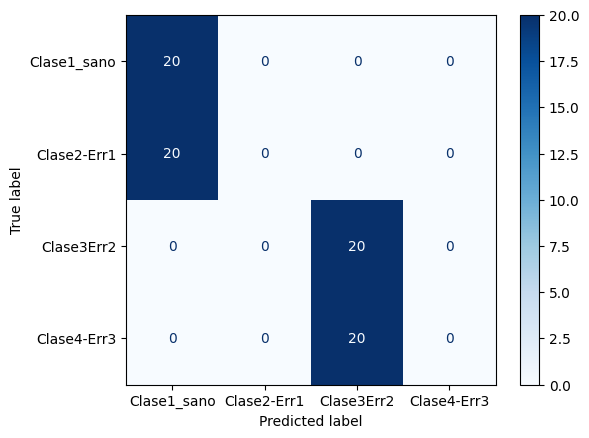
\includegraphics[keepaspectratio]{practica1_files/figure-pdf/cell-3-output-2.png}}

\begin{verbatim}
Matriz de confusión para Árbol de Decisión sin PCA:
Exactitud (Accuracy): 0.5000
Precision (Precision): 0.2500
Sensibilidad (Recall): 0.5000
Puntaje F1 (F1-score): 0.3333
\end{verbatim}

\begin{verbatim}
c:\Users\CuentaTemporal\miniconda3\envs\nn\lib\site-packages\sklearn\metrics\_classification.py:1706: UndefinedMetricWarning: Precision is ill-defined and being set to 0.0 in labels with no predicted samples. Use `zero_division` parameter to control this behavior.
  _warn_prf(average, modifier, f"{metric.capitalize()} is", result.shape[0])
\end{verbatim}

\begin{Shaded}
\begin{Highlighting}[]
\CommentTok{\#Con PCA }
\NormalTok{scaler }\OperatorTok{=}\NormalTok{ StandardScaler()}
\NormalTok{X\_scaled }\OperatorTok{=}\NormalTok{ scaler.fit\_transform(X)}
\NormalTok{pca }\OperatorTok{=}\NormalTok{ PCA(n\_components}\OperatorTok{=}\FloatTok{0.95}\NormalTok{)  }\CommentTok{\# Mantener el 95\% de la varianza}
\NormalTok{X\_pca }\OperatorTok{=}\NormalTok{ pca.fit\_transform(X\_scaled)}
\NormalTok{X\_train, X\_test, y\_train, y\_test }\OperatorTok{=}
\NormalTok{  train\_test\_split(X\_pca, y, test\_size}\OperatorTok{=}\FloatTok{0.2}\NormalTok{, random\_state}\OperatorTok{=}\DecValTok{42}\NormalTok{, stratify}\OperatorTok{=}\NormalTok{y)}
\CommentTok{\# Entrenar el modelo de Árbol de Decisión}
\NormalTok{decision\_tree }\OperatorTok{=}
\NormalTok{  DecisionTreeClassifier(random\_state}\OperatorTok{=}\DecValTok{42}\NormalTok{, max\_depth}\OperatorTok{=}\DecValTok{1}\NormalTok{, min\_samples\_split}\OperatorTok{=}\DecValTok{2}\NormalTok{, min\_samples\_leaf}\OperatorTok{=}\DecValTok{1}\NormalTok{)}
\NormalTok{decision\_tree.fit(X\_train, y\_train)}
\CommentTok{\# Predecir y evaluar}
\NormalTok{y\_pred }\OperatorTok{=}\NormalTok{ decision\_tree.predict(X\_test)}
\NormalTok{cm }\OperatorTok{=}\NormalTok{ confusion\_matrix(y\_test, y\_pred)}
\NormalTok{disp }\OperatorTok{=}\NormalTok{ ConfusionMatrixDisplay(}
\NormalTok{  confusion\_matrix}\OperatorTok{=}\NormalTok{cm,}
\NormalTok{  display\_labels}\OperatorTok{=}\NormalTok{decision\_tree.classes\_}
\NormalTok{)}
\NormalTok{disp.plot(cmap}\OperatorTok{=}\StringTok{\textquotesingle{}Blues\textquotesingle{}}\NormalTok{)}
\NormalTok{plt.show()}
\BuiltInTok{print}\NormalTok{(}\StringTok{"Matriz de confusión para Árbol de Decisión con PCA:"}\NormalTok{)}

\NormalTok{accuracy }\OperatorTok{=}\NormalTok{ accuracy\_score(y\_test, y\_pred)}
\BuiltInTok{print}\NormalTok{(}\SpecialStringTok{f\textquotesingle{}Exactitud (Accuracy): }\SpecialCharTok{\{}\NormalTok{accuracy}\SpecialCharTok{:.4f\}}\SpecialStringTok{\textquotesingle{}}\NormalTok{)}

\NormalTok{precision }\OperatorTok{=}\NormalTok{ precision\_score(y\_test, y\_pred, average}\OperatorTok{=}\StringTok{\textquotesingle{}weighted\textquotesingle{}}\NormalTok{)}
\NormalTok{recall }\OperatorTok{=}\NormalTok{ recall\_score(y\_test, y\_pred, average}\OperatorTok{=}\StringTok{\textquotesingle{}weighted\textquotesingle{}}\NormalTok{)}
\NormalTok{f1 }\OperatorTok{=}\NormalTok{ f1\_score(y\_test, y\_pred, average}\OperatorTok{=}\StringTok{\textquotesingle{}weighted\textquotesingle{}}\NormalTok{)}

\BuiltInTok{print}\NormalTok{(}\SpecialStringTok{f\textquotesingle{}Precision (Precision): }\SpecialCharTok{\{}\NormalTok{precision}\SpecialCharTok{:.4f\}}\SpecialStringTok{\textquotesingle{}}\NormalTok{)}
\BuiltInTok{print}\NormalTok{(}\SpecialStringTok{f\textquotesingle{}Sensibilidad (Recall): }\SpecialCharTok{\{}\NormalTok{recall}\SpecialCharTok{:.4f\}}\SpecialStringTok{\textquotesingle{}}\NormalTok{)}
\BuiltInTok{print}\NormalTok{(}\SpecialStringTok{f\textquotesingle{}Puntaje F1 (F1{-}score): }\SpecialCharTok{\{}\NormalTok{f1}\SpecialCharTok{:.4f\}}\SpecialStringTok{\textquotesingle{}}\NormalTok{)}
\end{Highlighting}
\end{Shaded}

\pandocbounded{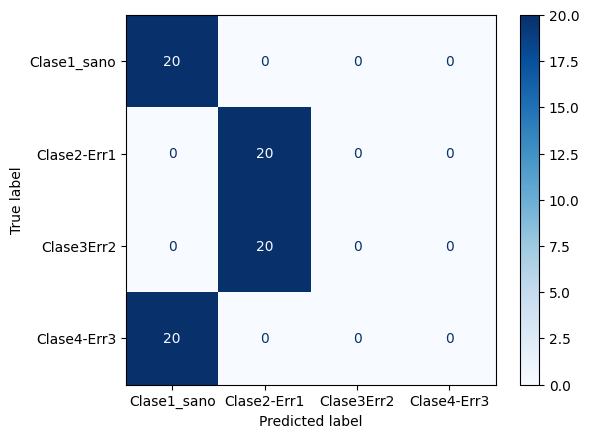
\includegraphics[keepaspectratio]{practica1_files/figure-pdf/cell-4-output-1.png}}

\begin{verbatim}
Matriz de confusión para Árbol de Decisión con PCA:
Exactitud (Accuracy): 0.5000
Precision (Precision): 0.2500
Sensibilidad (Recall): 0.5000
Puntaje F1 (F1-score): 0.3333
\end{verbatim}

\begin{verbatim}
c:\Users\CuentaTemporal\miniconda3\envs\nn\lib\site-packages\sklearn\metrics\_classification.py:1706: UndefinedMetricWarning: Precision is ill-defined and being set to 0.0 in labels with no predicted samples. Use `zero_division` parameter to control this behavior.
  _warn_prf(average, modifier, f"{metric.capitalize()} is", result.shape[0])
\end{verbatim}

\begin{Shaded}
\begin{Highlighting}[]
\CommentTok{\#Random Forest sin PCA}
\NormalTok{rf }\OperatorTok{=}\NormalTok{ RandomForestClassifier(}
\NormalTok{  random\_state}\OperatorTok{=}\DecValTok{42}\NormalTok{, n\_estimators}\OperatorTok{=}\DecValTok{100}\NormalTok{,}
\NormalTok{  max\_depth}\OperatorTok{=}\DecValTok{1}\NormalTok{,}
\NormalTok{  min\_samples\_split}\OperatorTok{=}\DecValTok{2}\NormalTok{,}
\NormalTok{  min\_samples\_leaf}\OperatorTok{=}\DecValTok{1}
\NormalTok{)}
\NormalTok{X\_train, X\_test, y\_train, y\_test }\OperatorTok{=}
\NormalTok{  train\_test\_split(X, y, test\_size}\OperatorTok{=}\FloatTok{0.2}\NormalTok{, random\_state}\OperatorTok{=}\DecValTok{42}\NormalTok{, stratify}\OperatorTok{=}\NormalTok{y)}
\NormalTok{rf.fit(X\_train, y\_train)}
\CommentTok{\# Predecir y evaluar}
\NormalTok{y\_pred }\OperatorTok{=}\NormalTok{ rf.predict(X\_test)}
\NormalTok{cm }\OperatorTok{=}\NormalTok{ confusion\_matrix(y\_test, y\_pred)}
\NormalTok{disp }\OperatorTok{=}\NormalTok{ ConfusionMatrixDisplay(confusion\_matrix}\OperatorTok{=}\NormalTok{cm, display\_labels}\OperatorTok{=}\NormalTok{rf.classes\_)}
\NormalTok{disp.plot(cmap}\OperatorTok{=}\StringTok{\textquotesingle{}Blues\textquotesingle{}}\NormalTok{)}
\NormalTok{plt.show()}
\BuiltInTok{print}\NormalTok{(}\StringTok{"Matriz de confusión para Random Forest sin PCA:"}\NormalTok{)}

\NormalTok{accuracy }\OperatorTok{=}\NormalTok{ accuracy\_score(y\_test, y\_pred)}
\BuiltInTok{print}\NormalTok{(}\SpecialStringTok{f\textquotesingle{}Exactitud (Accuracy): }\SpecialCharTok{\{}\NormalTok{accuracy}\SpecialCharTok{:.4f\}}\SpecialStringTok{\textquotesingle{}}\NormalTok{)}

\NormalTok{precision }\OperatorTok{=}\NormalTok{ precision\_score(y\_test, y\_pred, average}\OperatorTok{=}\StringTok{\textquotesingle{}weighted\textquotesingle{}}\NormalTok{)}
\NormalTok{recall }\OperatorTok{=}\NormalTok{ recall\_score(y\_test, y\_pred, average}\OperatorTok{=}\StringTok{\textquotesingle{}weighted\textquotesingle{}}\NormalTok{)}
\NormalTok{f1 }\OperatorTok{=}\NormalTok{ f1\_score(y\_test, y\_pred, average}\OperatorTok{=}\StringTok{\textquotesingle{}weighted\textquotesingle{}}\NormalTok{)}

\BuiltInTok{print}\NormalTok{(}\SpecialStringTok{f\textquotesingle{}Precision (Precision): }\SpecialCharTok{\{}\NormalTok{precision}\SpecialCharTok{:.4f\}}\SpecialStringTok{\textquotesingle{}}\NormalTok{)}
\BuiltInTok{print}\NormalTok{(}\SpecialStringTok{f\textquotesingle{}Sensibilidad (Recall): }\SpecialCharTok{\{}\NormalTok{recall}\SpecialCharTok{:.4f\}}\SpecialStringTok{\textquotesingle{}}\NormalTok{)}
\BuiltInTok{print}\NormalTok{(}\SpecialStringTok{f\textquotesingle{}Puntaje F1 (F1{-}score): }\SpecialCharTok{\{}\NormalTok{f1}\SpecialCharTok{:.4f\}}\SpecialStringTok{\textquotesingle{}}\NormalTok{)}
\end{Highlighting}
\end{Shaded}

\pandocbounded{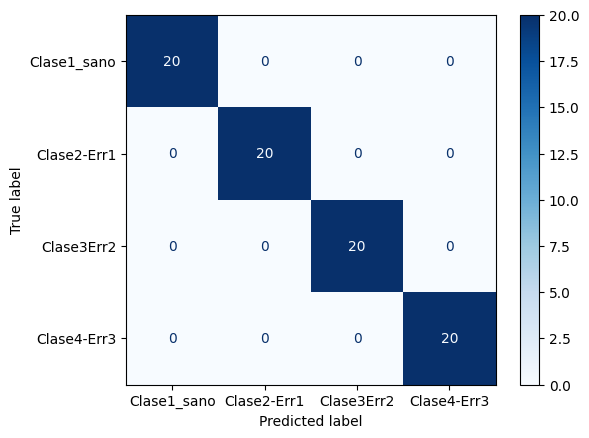
\includegraphics[keepaspectratio]{practica1_files/figure-pdf/cell-5-output-1.png}}

\begin{verbatim}
Matriz de confusión para Random Forest sin PCA:
Exactitud (Accuracy): 1.0000
Precision (Precision): 1.0000
Sensibilidad (Recall): 1.0000
Puntaje F1 (F1-score): 1.0000
\end{verbatim}

\begin{Shaded}
\begin{Highlighting}[]
\CommentTok{\#Random Forest con PCA}
\NormalTok{rf }\OperatorTok{=}\NormalTok{ RandomForestClassifier(}
\NormalTok{  random\_state}\OperatorTok{=}\DecValTok{42}\NormalTok{,}
\NormalTok{  n\_estimators}\OperatorTok{=}\DecValTok{100}\NormalTok{,}
\NormalTok{  max\_depth}\OperatorTok{=}\DecValTok{1}\NormalTok{,}
\NormalTok{  min\_samples\_split}\OperatorTok{=}\DecValTok{2}\NormalTok{,}
\NormalTok{  min\_samples\_leaf}\OperatorTok{=}\DecValTok{1}
\NormalTok{)}
\NormalTok{X\_train, X\_test, y\_train, y\_test }\OperatorTok{=} 
\NormalTok{  rain\_test\_split(X\_pca, y, test\_size}\OperatorTok{=}\FloatTok{0.2}\NormalTok{, random\_state}\OperatorTok{=}\DecValTok{42}\NormalTok{, stratify}\OperatorTok{=}\NormalTok{y)}
\NormalTok{rf.fit(X\_train, y\_train)}
\CommentTok{\# Predecir y evaluar}
\NormalTok{y\_pred }\OperatorTok{=}\NormalTok{ rf.predict(X\_test)}
\NormalTok{cm }\OperatorTok{=}\NormalTok{ confusion\_matrix(y\_test, y\_pred)}
\NormalTok{disp }\OperatorTok{=}\NormalTok{ ConfusionMatrixDisplay(confusion\_matrix}\OperatorTok{=}\NormalTok{cm, display\_labels}\OperatorTok{=}\NormalTok{rf.classes\_)}
\NormalTok{disp.plot(cmap}\OperatorTok{=}\StringTok{\textquotesingle{}Blues\textquotesingle{}}\NormalTok{)}
\NormalTok{plt.show()}
\BuiltInTok{print}\NormalTok{(}\StringTok{"Matriz de confusión para Random Forest con PCA:"}\NormalTok{)}

\NormalTok{accuracy }\OperatorTok{=}\NormalTok{ accuracy\_score(y\_test, y\_pred)}
\BuiltInTok{print}\NormalTok{(}\SpecialStringTok{f\textquotesingle{}Exactitud (Accuracy): }\SpecialCharTok{\{}\NormalTok{accuracy}\SpecialCharTok{:.4f\}}\SpecialStringTok{\textquotesingle{}}\NormalTok{)}

\NormalTok{precision }\OperatorTok{=}\NormalTok{ precision\_score(y\_test, y\_pred, average}\OperatorTok{=}\StringTok{\textquotesingle{}weighted\textquotesingle{}}\NormalTok{)}
\NormalTok{recall }\OperatorTok{=}\NormalTok{ recall\_score(y\_test, y\_pred, average}\OperatorTok{=}\StringTok{\textquotesingle{}weighted\textquotesingle{}}\NormalTok{)}
\NormalTok{f1 }\OperatorTok{=}\NormalTok{ f1\_score(y\_test, y\_pred, average}\OperatorTok{=}\StringTok{\textquotesingle{}weighted\textquotesingle{}}\NormalTok{)}

\BuiltInTok{print}\NormalTok{(}\SpecialStringTok{f\textquotesingle{}Precision (Precision): }\SpecialCharTok{\{}\NormalTok{precision}\SpecialCharTok{:.4f\}}\SpecialStringTok{\textquotesingle{}}\NormalTok{)}
\BuiltInTok{print}\NormalTok{(}\SpecialStringTok{f\textquotesingle{}Sensibilidad (Recall): }\SpecialCharTok{\{}\NormalTok{recall}\SpecialCharTok{:.4f\}}\SpecialStringTok{\textquotesingle{}}\NormalTok{)}
\BuiltInTok{print}\NormalTok{(}\SpecialStringTok{f\textquotesingle{}Puntaje F1 (F1{-}score): }\SpecialCharTok{\{}\NormalTok{f1}\SpecialCharTok{:.4f\}}\SpecialStringTok{\textquotesingle{}}\NormalTok{)}
\end{Highlighting}
\end{Shaded}

\pandocbounded{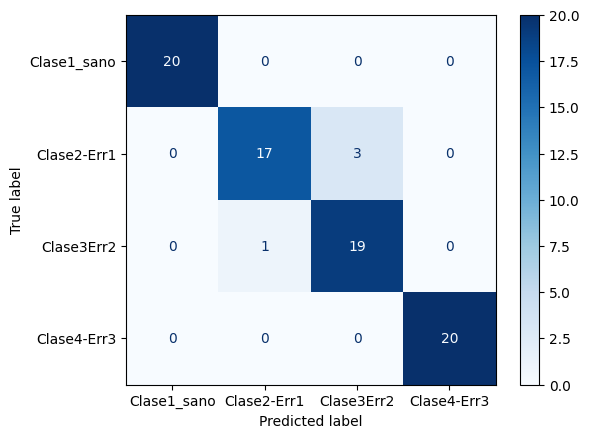
\includegraphics[keepaspectratio]{practica1_files/figure-pdf/cell-6-output-1.png}}

\begin{verbatim}
Matriz de confusión para Random Forest con PCA:
Exactitud (Accuracy): 0.9500
Precision (Precision): 0.9520
Sensibilidad (Recall): 0.9500
Puntaje F1 (F1-score): 0.9499
\end{verbatim}

\begin{Shaded}
\begin{Highlighting}[]
\CommentTok{\#Random Forest con LDA}
\CommentTok{\#Con LDA}
\ImportTok{from}\NormalTok{ sklearn.discriminant\_analysis }\ImportTok{import}\NormalTok{ LinearDiscriminantAnalysis }\ImportTok{as}\NormalTok{ LDA}
\NormalTok{lda }\OperatorTok{=}\NormalTok{ LDA()}
\NormalTok{X\_lda }\OperatorTok{=}\NormalTok{ lda.fit\_transform(X,y)}


\NormalTok{rf }\OperatorTok{=}\NormalTok{ RandomForestClassifier(}
\NormalTok{  random\_state}\OperatorTok{=}\DecValTok{42}\NormalTok{,}
\NormalTok{  n\_estimators}\OperatorTok{=}\DecValTok{100}\NormalTok{,}
\NormalTok{  max\_depth}\OperatorTok{=}\DecValTok{1}\NormalTok{,}
\NormalTok{  min\_samples\_split}\OperatorTok{=}\DecValTok{2}\NormalTok{,}
\NormalTok{  min\_samples\_leaf}\OperatorTok{=}\DecValTok{1}
\NormalTok{)}
\NormalTok{X\_train, X\_test, y\_train, y\_test }\OperatorTok{=}
\NormalTok{  train\_test\_split(X\_lda, y, test\_size}\OperatorTok{=}\FloatTok{0.2}\NormalTok{, random\_state}\OperatorTok{=}\DecValTok{42}\NormalTok{, stratify}\OperatorTok{=}\NormalTok{y)}
\NormalTok{rf.fit(X\_train, y\_train)}
\CommentTok{\# Predecir y evaluar}
\NormalTok{y\_pred }\OperatorTok{=}\NormalTok{ rf.predict(X\_test)}
\NormalTok{cm }\OperatorTok{=}\NormalTok{ confusion\_matrix(y\_test, y\_pred)}
\NormalTok{disp }\OperatorTok{=}\NormalTok{ ConfusionMatrixDisplay(confusion\_matrix}\OperatorTok{=}\NormalTok{cm, display\_labels}\OperatorTok{=}\NormalTok{rf.classes\_)}
\NormalTok{disp.plot(cmap}\OperatorTok{=}\StringTok{\textquotesingle{}Blues\textquotesingle{}}\NormalTok{)}
\NormalTok{plt.show()}
\BuiltInTok{print}\NormalTok{(}\StringTok{"Matriz de confusión para Random Forest con LDA:"}\NormalTok{)}

\NormalTok{accuracy }\OperatorTok{=}\NormalTok{ accuracy\_score(y\_test, y\_pred)}
\BuiltInTok{print}\NormalTok{(}\SpecialStringTok{f\textquotesingle{}Exactitud (Accuracy): }\SpecialCharTok{\{}\NormalTok{accuracy}\SpecialCharTok{:.4f\}}\SpecialStringTok{\textquotesingle{}}\NormalTok{)}

\NormalTok{precision }\OperatorTok{=}\NormalTok{ precision\_score(y\_test, y\_pred, average}\OperatorTok{=}\StringTok{\textquotesingle{}weighted\textquotesingle{}}\NormalTok{)}
\NormalTok{recall }\OperatorTok{=}\NormalTok{ recall\_score(y\_test, y\_pred, average}\OperatorTok{=}\StringTok{\textquotesingle{}weighted\textquotesingle{}}\NormalTok{)}
\NormalTok{f1 }\OperatorTok{=}\NormalTok{ f1\_score(y\_test, y\_pred, average}\OperatorTok{=}\StringTok{\textquotesingle{}weighted\textquotesingle{}}\NormalTok{)}

\BuiltInTok{print}\NormalTok{(}\SpecialStringTok{f\textquotesingle{}Precision (Precision): }\SpecialCharTok{\{}\NormalTok{precision}\SpecialCharTok{:.4f\}}\SpecialStringTok{\textquotesingle{}}\NormalTok{)}
\BuiltInTok{print}\NormalTok{(}\SpecialStringTok{f\textquotesingle{}Sensibilidad (Recall): }\SpecialCharTok{\{}\NormalTok{recall}\SpecialCharTok{:.4f\}}\SpecialStringTok{\textquotesingle{}}\NormalTok{)}
\BuiltInTok{print}\NormalTok{(}\SpecialStringTok{f\textquotesingle{}Puntaje F1 (F1{-}score): }\SpecialCharTok{\{}\NormalTok{f1}\SpecialCharTok{:.4f\}}\SpecialStringTok{\textquotesingle{}}\NormalTok{)}
\end{Highlighting}
\end{Shaded}

\pandocbounded{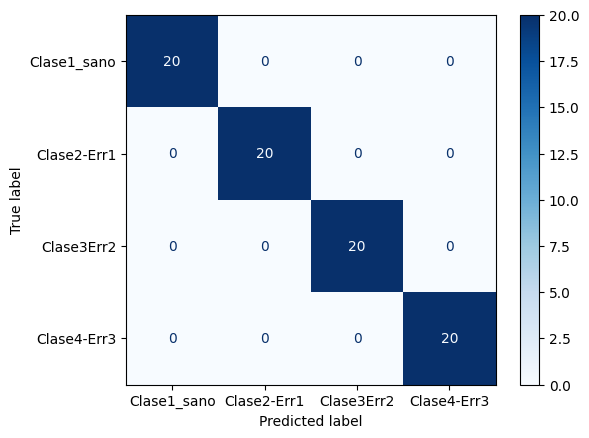
\includegraphics[keepaspectratio]{practica1_files/figure-pdf/cell-7-output-1.png}}

\begin{verbatim}
Matriz de confusión para Random Forest con LDA:
Exactitud (Accuracy): 1.0000
Precision (Precision): 1.0000
Sensibilidad (Recall): 1.0000
Puntaje F1 (F1-score): 1.0000
\end{verbatim}

\begin{Shaded}
\begin{Highlighting}[]
\CommentTok{\#AdaBoost sin PCA}
\NormalTok{clf }\OperatorTok{=}\NormalTok{ DecisionTreeClassifier(}
\NormalTok{  random\_state}\OperatorTok{=}\DecValTok{42}\NormalTok{ ,max\_depth}\OperatorTok{=}\DecValTok{1}\NormalTok{,}
\NormalTok{  min\_samples\_split}\OperatorTok{=}\DecValTok{2}\NormalTok{,}
\NormalTok{  min\_samples\_leaf}\OperatorTok{=}\DecValTok{1}
\NormalTok{)}
\NormalTok{ada }\OperatorTok{=}\NormalTok{ AdaBoostClassifier(estimator}\OperatorTok{=}\NormalTok{clf, n\_estimators}\OperatorTok{=}\DecValTok{50}\NormalTok{, random\_state}\OperatorTok{=}\DecValTok{42}\NormalTok{)}
\NormalTok{X\_train, X\_test, y\_train, y\_test }\OperatorTok{=}
\NormalTok{  train\_test\_split(X, y, test\_size}\OperatorTok{=}\FloatTok{0.2}\NormalTok{, random\_state}\OperatorTok{=}\DecValTok{42}\NormalTok{, stratify}\OperatorTok{=}\NormalTok{y)}
\NormalTok{ada.fit(X\_train, y\_train)}
\CommentTok{\# Predecir y evaluar}
\NormalTok{y\_pred }\OperatorTok{=}\NormalTok{ ada.predict(X\_test)}
\NormalTok{cm }\OperatorTok{=}\NormalTok{ confusion\_matrix(y\_test, y\_pred)}
\NormalTok{disp }\OperatorTok{=}\NormalTok{ ConfusionMatrixDisplay(confusion\_matrix}\OperatorTok{=}\NormalTok{cm, display\_labels}\OperatorTok{=}\NormalTok{ada.classes\_)}
\NormalTok{disp.plot(cmap}\OperatorTok{=}\StringTok{\textquotesingle{}Blues\textquotesingle{}}\NormalTok{)}
\NormalTok{plt.show()}
\BuiltInTok{print}\NormalTok{(}\StringTok{"Matriz de confusión para AdaBoost sin PCA:"}\NormalTok{)}

\NormalTok{accuracy }\OperatorTok{=}\NormalTok{ accuracy\_score(y\_test, y\_pred)}
\BuiltInTok{print}\NormalTok{(}\SpecialStringTok{f\textquotesingle{}Exactitud (Accuracy): }\SpecialCharTok{\{}\NormalTok{accuracy}\SpecialCharTok{:.4f\}}\SpecialStringTok{\textquotesingle{}}\NormalTok{)}

\NormalTok{precision }\OperatorTok{=}\NormalTok{ precision\_score(y\_test, y\_pred, average}\OperatorTok{=}\StringTok{\textquotesingle{}weighted\textquotesingle{}}\NormalTok{)}
\NormalTok{recall }\OperatorTok{=}\NormalTok{ recall\_score(y\_test, y\_pred, average}\OperatorTok{=}\StringTok{\textquotesingle{}weighted\textquotesingle{}}\NormalTok{)}
\NormalTok{f1 }\OperatorTok{=}\NormalTok{ f1\_score(y\_test, y\_pred, average}\OperatorTok{=}\StringTok{\textquotesingle{}weighted\textquotesingle{}}\NormalTok{)}

\BuiltInTok{print}\NormalTok{(}\SpecialStringTok{f\textquotesingle{}Precision (Precision): }\SpecialCharTok{\{}\NormalTok{precision}\SpecialCharTok{:.4f\}}\SpecialStringTok{\textquotesingle{}}\NormalTok{)}
\BuiltInTok{print}\NormalTok{(}\SpecialStringTok{f\textquotesingle{}Sensibilidad (Recall): }\SpecialCharTok{\{}\NormalTok{recall}\SpecialCharTok{:.4f\}}\SpecialStringTok{\textquotesingle{}}\NormalTok{)}
\BuiltInTok{print}\NormalTok{(}\SpecialStringTok{f\textquotesingle{}Puntaje F1 (F1{-}score): }\SpecialCharTok{\{}\NormalTok{f1}\SpecialCharTok{:.4f\}}\SpecialStringTok{\textquotesingle{}}\NormalTok{)}
\end{Highlighting}
\end{Shaded}

\pandocbounded{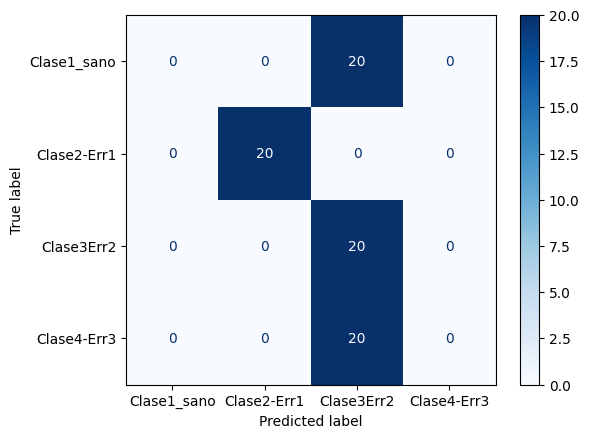
\includegraphics[keepaspectratio]{practica1_files/figure-pdf/cell-8-output-1.png}}

\begin{verbatim}
Matriz de confusión para AdaBoost sin PCA:
Exactitud (Accuracy): 0.5000
Precision (Precision): 0.3333
Sensibilidad (Recall): 0.5000
Puntaje F1 (F1-score): 0.3750
\end{verbatim}

\begin{verbatim}
c:\Users\CuentaTemporal\miniconda3\envs\nn\lib\site-packages\sklearn\metrics\_classification.py:1706: UndefinedMetricWarning: Precision is ill-defined and being set to 0.0 in labels with no predicted samples. Use `zero_division` parameter to control this behavior.
  _warn_prf(average, modifier, f"{metric.capitalize()} is", result.shape[0])
\end{verbatim}

\begin{Shaded}
\begin{Highlighting}[]
\CommentTok{\#AdaBoost con PCA}
\NormalTok{clf }\OperatorTok{=}\NormalTok{ DecisionTreeClassifier(}
\NormalTok{  random\_state}\OperatorTok{=}\DecValTok{42}\NormalTok{ ,max\_depth}\OperatorTok{=}\DecValTok{1}\NormalTok{,}
\NormalTok{  min\_samples\_split}\OperatorTok{=}\DecValTok{2}\NormalTok{,}
\NormalTok{  min\_samples\_leaf}\OperatorTok{=}\DecValTok{1}
\NormalTok{)}
\NormalTok{ada }\OperatorTok{=}\NormalTok{ AdaBoostClassifier(estimator}\OperatorTok{=}\NormalTok{clf, n\_estimators}\OperatorTok{=}\DecValTok{50}\NormalTok{, random\_state}\OperatorTok{=}\DecValTok{42}\NormalTok{)}
\NormalTok{X\_train, X\_test, y\_train, y\_test }\OperatorTok{=}
\NormalTok{train\_test\_split(X\_pca, y, test\_size}\OperatorTok{=}\FloatTok{0.2}\NormalTok{, random\_state}\OperatorTok{=}\DecValTok{42}\NormalTok{, stratify}\OperatorTok{=}\NormalTok{y)}
\NormalTok{ada.fit(X\_train, y\_train)}
\CommentTok{\# Predecir y evaluar}
\NormalTok{y\_pred }\OperatorTok{=}\NormalTok{ ada.predict(X\_test)}
\NormalTok{cm }\OperatorTok{=}\NormalTok{ confusion\_matrix(y\_test, y\_pred)}
\NormalTok{disp }\OperatorTok{=}\NormalTok{ ConfusionMatrixDisplay(confusion\_matrix}\OperatorTok{=}\NormalTok{cm, display\_labels}\OperatorTok{=}\NormalTok{ada.classes\_)}
\NormalTok{disp.plot(cmap}\OperatorTok{=}\StringTok{\textquotesingle{}Blues\textquotesingle{}}\NormalTok{)}
\NormalTok{plt.show()}
\BuiltInTok{print}\NormalTok{(}\StringTok{"Matriz de confusión para AdaBoost con PCA:"}\NormalTok{)}

\NormalTok{accuracy }\OperatorTok{=}\NormalTok{ accuracy\_score(y\_test, y\_pred)}
\BuiltInTok{print}\NormalTok{(}\SpecialStringTok{f\textquotesingle{}Exactitud (Accuracy): }\SpecialCharTok{\{}\NormalTok{accuracy}\SpecialCharTok{:.4f\}}\SpecialStringTok{\textquotesingle{}}\NormalTok{)}

\NormalTok{precision }\OperatorTok{=}\NormalTok{ precision\_score(y\_test, y\_pred, average}\OperatorTok{=}\StringTok{\textquotesingle{}weighted\textquotesingle{}}\NormalTok{)}
\NormalTok{recall }\OperatorTok{=}\NormalTok{ recall\_score(y\_test, y\_pred, average}\OperatorTok{=}\StringTok{\textquotesingle{}weighted\textquotesingle{}}\NormalTok{)}
\NormalTok{f1 }\OperatorTok{=}\NormalTok{ f1\_score(y\_test, y\_pred, average}\OperatorTok{=}\StringTok{\textquotesingle{}weighted\textquotesingle{}}\NormalTok{)}

\BuiltInTok{print}\NormalTok{(}\SpecialStringTok{f\textquotesingle{}Precision (Precision): }\SpecialCharTok{\{}\NormalTok{precision}\SpecialCharTok{:.4f\}}\SpecialStringTok{\textquotesingle{}}\NormalTok{)}
\BuiltInTok{print}\NormalTok{(}\SpecialStringTok{f\textquotesingle{}Sensibilidad (Recall): }\SpecialCharTok{\{}\NormalTok{recall}\SpecialCharTok{:.4f\}}\SpecialStringTok{\textquotesingle{}}\NormalTok{)}
\BuiltInTok{print}\NormalTok{(}\SpecialStringTok{f\textquotesingle{}Puntaje F1 (F1{-}score): }\SpecialCharTok{\{}\NormalTok{f1}\SpecialCharTok{:.4f\}}\SpecialStringTok{\textquotesingle{}}\NormalTok{)}
\end{Highlighting}
\end{Shaded}

\pandocbounded{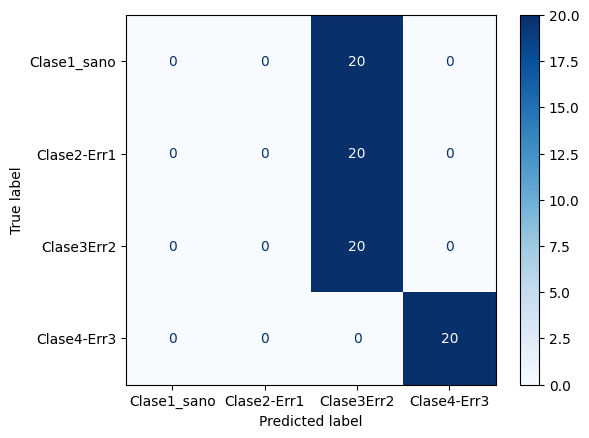
\includegraphics[keepaspectratio]{practica1_files/figure-pdf/cell-9-output-1.png}}

\begin{verbatim}
Matriz de confusión para AdaBoost con PCA:
Exactitud (Accuracy): 0.5000
Precision (Precision): 0.3333
Sensibilidad (Recall): 0.5000
Puntaje F1 (F1-score): 0.3750
\end{verbatim}

\begin{verbatim}
c:\Users\CuentaTemporal\miniconda3\envs\nn\lib\site-packages\sklearn\metrics\_classification.py:1706: UndefinedMetricWarning: Precision is ill-defined and being set to 0.0 in labels with no predicted samples. Use `zero_division` parameter to control this behavior.
  _warn_prf(average, modifier, f"{metric.capitalize()} is", result.shape[0])
\end{verbatim}




\end{document}
